\documentclass[11pt]{article}
\usepackage[margin=0.85in]{geometry}
\usepackage{amsmath,amssymb,graphicx,hyperref}
\setlength{\parindent}{0pt}\setlength{\parskip}{6pt}
\setlength{\emergencystretch}{3em}
\begin{document}
{\Large Actual norm matrices and bounded coordinate families}\\
November 13, 2026. Unsigned producer evidence [pcc:unverified].

\textbf{Actual matrix connection.} For polynomial families $A_i,B_i$ and a
field-linear polynomial functional $\mu$, define
\[
 E_{ik}=A_iA_k-fB_iB_k,\quad D_{ik}=\mu(E_{ik}),\qquad
 (C_j)_{ik}=[X^j]E_{ik}-[X^d]E_{ik}\,[X^j]G,
\]
where $d=\operatorname{natDegree}G$. The actual moment matrix is symmetric.
For $A_w=\sum_iw_iA_i$, $B_w=\sum_iw_iB_i$, $N_w=A_w^2-fB_w^2$,
Lean establishes
\[
 w^TDw=\mu(N_w),\quad w^TC_jw=[X^j]N_w-[X^d]N_w\,[X^j]G.
\]
If $G$ is monic, $\mu(G)=0$ and the entry degrees are bounded by $d$, the
preceding functional theorem gives the exact entrywise matrix identity
\[
 D=\sum_{j<d}\mu(X^j)C_j.
\]
The final actual-witness theorem derives $\mu(G)=0$ and the entry bounds;
it does not assume matrix-pencil membership or numerical rank.

\textbf{Canonical full chart.} Supplied monic $F,H,G$ satisfy
\[
 UF+V(fH)=1,\quad(\alpha F)^2-f(\beta H)^2=cG,\quad c\ne0.
\]
Let $a=\deg F=b+2$, $b=\deg H>0$, $\deg G=2a$, $\deg f\le3$.
Use the actual quotient moment from the preceding theorem and the product
monomial basis of the polynomial spaces of degrees $<a+1$ and $<b+1$.
The first and second components supply the families. Their bounds and
completeness are proved: every bounded pair $(P,Q)$ is $(A_w,B_w)$ for some
common coordinate vector $w$. These canonical matrices satisfy the identity.

\begin{center}
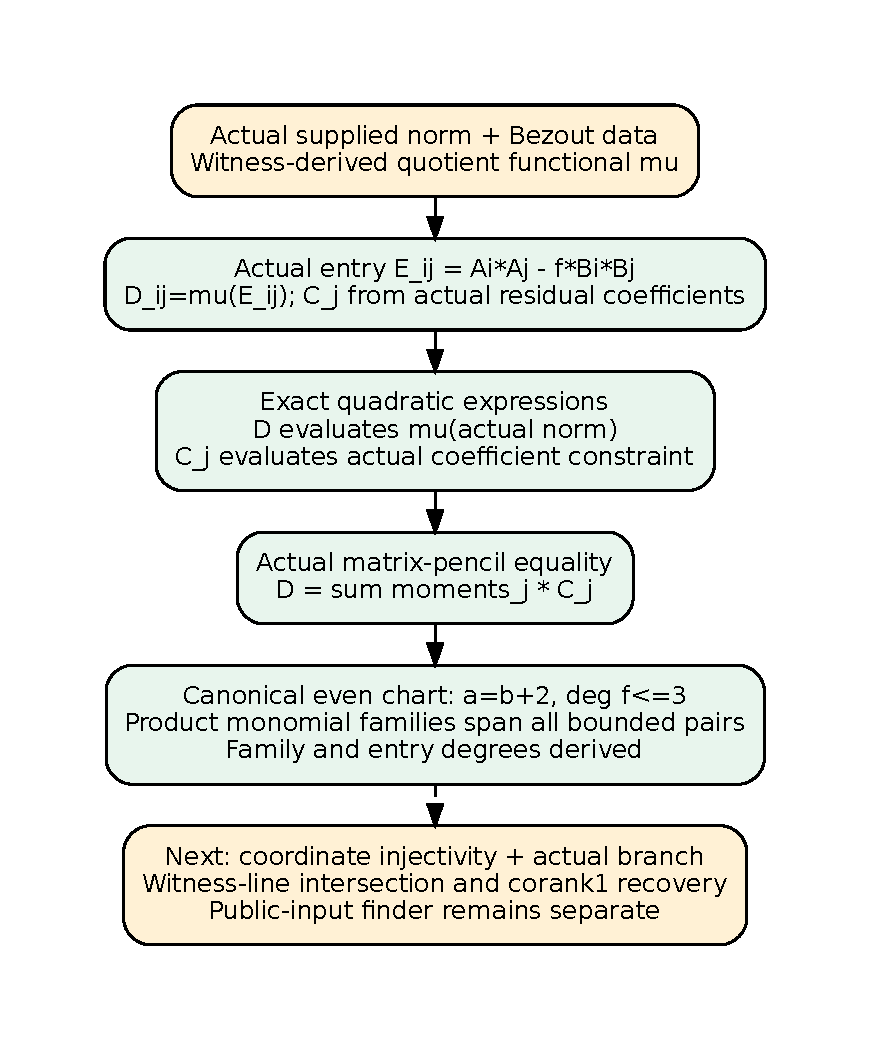
\includegraphics[width=0.9\linewidth,height=0.34\textheight,keepaspectratio]{matrix.pdf}
\end{center}

\newpage
{\Large Exact scope, checks and next transfer}

\textbf{Formal source.} \path{NormMomentMatrix.lean}, frozen source commit
\path{cc5c9651a}. Ten declarations cover symmetry, actual norm/coefficient
quadratics, matrix-pencil equality, family/entry degrees, bounded-pair
completeness and the full even chart. Main declarations include
\path{matrixPencil}, \path{familiesComplete} and \path{canonicalMatrixPencil}.
The accompanying Markdown report maps every result to its exact source and
hypotheses; ten producer bindings remain unsigned. No characteristic or
separability restriction is introduced by this component.

\textbf{Checks.} Lean4.35.0 and unchanged pinned dependencies. Build006
passes3149 jobs; printed axioms are standard foundations only. Actual-source
audit covers120 declarations with zero failing and zero additional trusted
axioms. Separate fresh import-inclusive replay exits0; its own completion
receipt is retained. No signed PCC verdict is claimed.

Build001 failed on intro applied to transpose equality and wrong function-sum
simplification for Matrix. Matrix ext/sum/smul declarations resolve those errors.
Build004 used unrestricted simp on projected basis reconstruction, reducing the
supplied equation to True; controlled product/submodule sum rewrites resolve
it. All failed and completed logs are retained. Earlier source hashes remain
unchanged.

\textbf{Supporting native record.} \path{IDC1h345f3824264d232a} is copied
unchanged from the preceding functional evidence. It checks the universal
commutative-ring norm polarization at the previously recorded32+32 points,
pinning that earlier exact source. No new native run is claimed. It does not
check arbitrary matrix sums, pencil membership or rank; those components use
their own Lean proofs. No Rust implementation changed in this round.

\textbf{Next transfer.} Prove coordinate injectivity and the arbitrary-pair
bilinear evaluation. Define the actual target branch, exhibit a radical vector
on which it is nonzero, and apply the earlier branch-test lemma. Compute the
scaled witness-line intersection and transfer its dimension to exact matrix
corank1; then apply guarded adjugate recovery with all nonzero/stationarity
guards. Exceptional charts and a public-input moment finder remain separate.
Current moments still use supplied witness data; the required $2^{o(n)}$ bit
search cost does not follow from matrix existence.

\textbf{Earlier completion proposal.} These matrices supply a concrete
rank-directed certificate form. Reachability through
$W_{\rm base}+C(T)H(T)$ and an efficient choice of its free coefficients remain
unestablished.

\textbf{Sources and resources.} Exact NormLift/NormDualPencil and functional
source; pinned Matrix sum/smul, DegreeLT product basis, basis reconstruction,
polynomial degree and product/submodule sum declarations. KB and conductor
unavailable; bounded fallback, no priority claim. No paid job, empirical
runtime/scaling campaign or budget override. Monthly isolab budget remains
exhausted. No benchmark/leaderboard/ecdb changes. Source-linked Markdown,
editable DOT/SVG, diagram PDF, this report and raw evidence accompany the result.
\end{document}
